\section{Methodology}
\label{sec:methods}

\subsection{Dataset}
\label{subsec:dataset}

The data



\subsection{Preprocessing}
\label{subsec:prepro}
The preprocessing of the images include: automatic selection of a region
of interest, image resampling to a resolution of $0.5 \times 0.5 \times 0.5$ mm, contours interpolation
using optical flow, bias correction using the N4ITK algorithm \cite{n4itk}, and
image normalization to an interval of [0,1].

The selection of the region of interested was proposed in \cite{anneke} and it 
consists of reducing the size of the three MRI series (axial, sagittal, and coronal)
by the intersection of its three corresponding rectangular prisms. The resampling
of the images is performed using linear interpolation with the ITK software \cite{itk}. 
The interpolation of the contours is performed in two dimensions fore each consecutives slices
of the contours. First, optical flow is obtained between the two slices using the  
Farneback method implementation in ITK. Then, the contours are modified following
the optical flow directions in a linear regression direction. Figure \ref{fig:of1} shows an
example of the resulting interpolated contour using the proposed method. 
\begin{figure}[h]
    \centering
    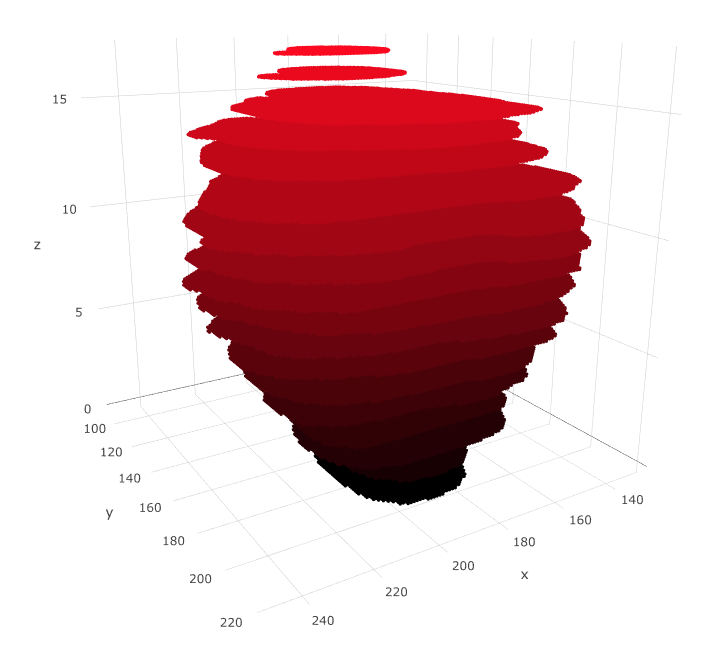
\includegraphics[totalheight=.15\textheight]{imgs/methodology/OF_1.png}
    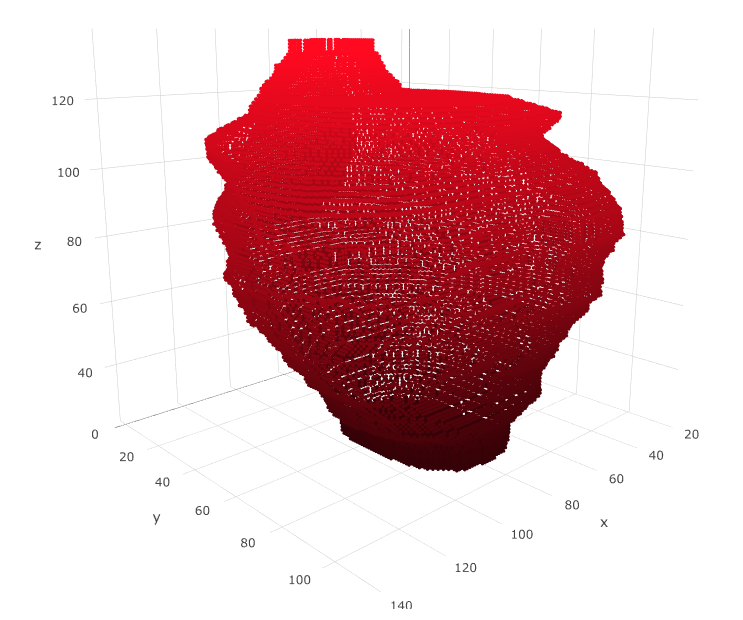
\includegraphics[totalheight=.15\textheight]{imgs/methodology/OF_2.png}
    \caption{Optical flow..}
    \label{fig:of1}
\end{figure}

\subsection{Proposed architecture}
The proposed 3D CNN consist of a multistream encoding stage and a decoding stage. Each
of the mulstistream inputs receive an MRI image series of the ROI with a resolution of
$168^3$. All convolutional layers use filter size of $3 \times 3 \times 3$ and
rectified linear unit (ReLu) as the activation function, with the exception
of the last layer which uses  $1 \times 1 \times 1$ filter size and Sigmoid function. 

\begin{figure*}[h]
    \centering
    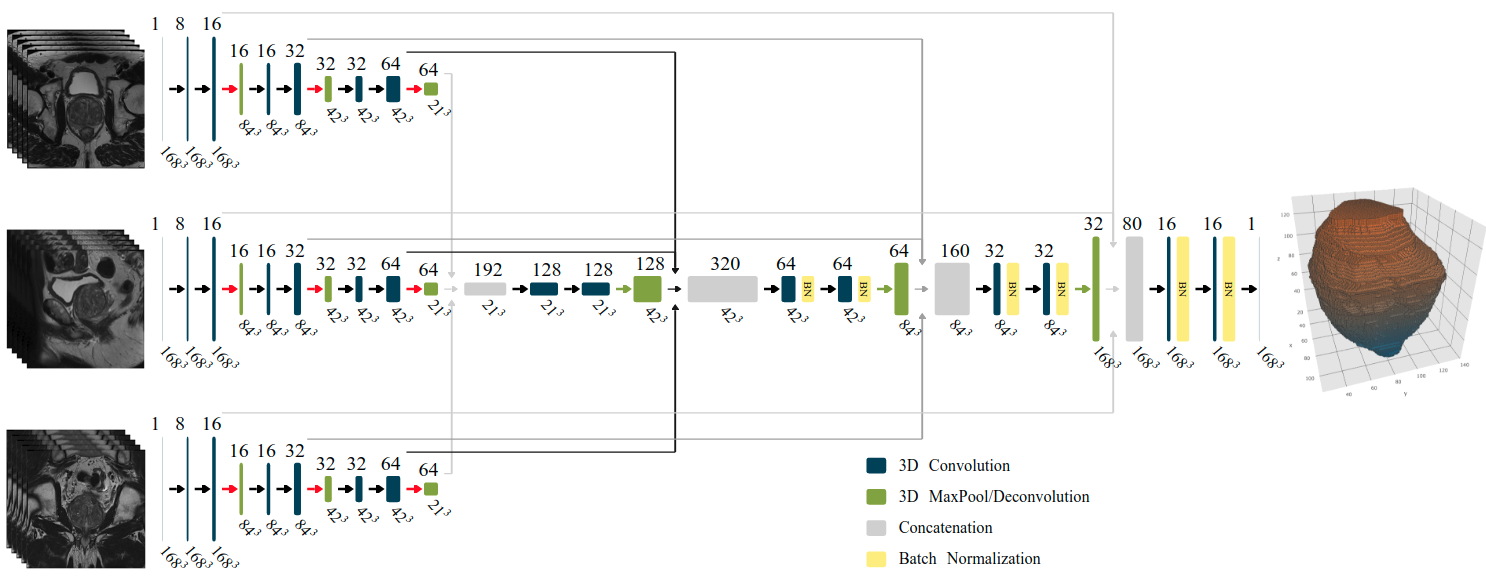
\includegraphics[totalheight=.3\textheight]{imgs/methodology/NN.png}
    \caption{Optical flow..}
    \label{fig:nn}
\end{figure*}

Some of the modifications proposed to the original architecture of Meyer et al. \cite{anneke} 
(based on teh 3D U-Net MISSREF)
are the reduced number of filters from 192 to 128 in the \emph{bottom} encoding layer, and
the addition of batch normalization after every convolutiional layer 
in the decoding phase. These adjustments reduce the training time on half without
loss of accuracy. 

\subsection{Training}
\label{subsec:training}
The selected optimization algorithm is Stochastic Gradient Descent (SGD) with a
learning rate $\alpha = 0.05$, momentum of 0.2 and decay of $10^{-7}$. The training is performed
for 1000 epochs, a batch size of 50, and an early stop mechanism for the validation
loss if not improved by $\delta = 0.001$ after 70 iterations. 

The loss function used for the training is the negative Dice similarity coefficient (DSC):
\begin{equation}
\text{Loss} = \frac{2 \sum_{i=1}^{N}p_it_i}{\sum_{i=1}^{N}p_i^2 + \sum_{i=1}^{N}t_i^2 + \varepsilon} 
\label{eq:dsc}
\end{equation}
%where N is the total number of voxels in the image, when training for prostate segmenation,
%and the number of voxels \textbf{inside} the prostate, when training for the PZ. The segmentation
%of the PZ assumes that we already know where the prostate is, so we do not take into
%account anything outside the prostate for the loss function. 
where N is the total number of voxels in the image, $p_i$ the voxel values for the 
prediction of the network, and $t_i$ the true voxel values of the prostate or PZ masks.

The dataset was split into 90\% for training and 10\% for
validation. Also, in order to compare the robustness of the models with respect to changes
in MRI vendor machines,  a distinct model was trained for the datasets GE (90
training and 10 validation) \& Siemens (295 training and 33 validation) and 
an additional model trained with the merged datasets (385 training and 43 validation). 

To analyze how 3D data augmentation can influence the sensitivity of the models
against different vendor machines, the models were also trained separated when
using data augmentation or not. The 3D data augmentation tested include flipping the
images in the sagittal axis,  shifting in any direction up to 10\%, and
bluring the images using Gaussian blur up to $\sigma = 3$. Each data augmentation
method is applied with a random chance of $1/3$.

Finally, a total number of 12 models were trained from the combination of 
three datasets, using or not data agumentation, and segmenting prostate or PZ. 
